% Teilaufgabe X

\section{Photostrom-Signal cw-Lasers mit mehreren longitudinalen Moden}
\label{sec:cwlaser}

Für Fundamentalmoden kann sich in einem Resonator mit ebenen Spiegeln für folgende Bedingung eine stehende Welle ausbilden:
\begin{gather}
    d = q \cdot \frac{\lambda}{2} \Rightarrow \nu = q \cdot \frac{c}{2d}~,
\end{gather}
wobei $\nu$ die zulässige Frequenz der $g$-ten Mode. Daraus folgt der Frequenzabstand:
\begin{gather}
    \boxed{\Delta \nu = \frac{c}{2d}}~,
\end{gather}
was auch freier Spektralbereich des Resonators genannt wird. Bei diesen Resonanzfrequenzen (Transveralmoden unterdrückt) kommt es dann zu Verlusten durch Reflexion, Streuung und Beugung. Dadurch können nur Frequenzen anschwingen, die über dem Schwellwert und im Verstärkerprofil des aktiven Mediums liegen, wobei die Laseremission dann aus all diesen Frequenzen $\nu$ besteht. Die Gesamtbreite der Laseremission hängt dabei von der Gesamtbreite des Laserprofils oberhalb des Schwellwerts [Abb. \ref{fig:cwlaser}]. \cite{DemtroederAtome}
\begin{center}
    \captionsetup{type=figure}
    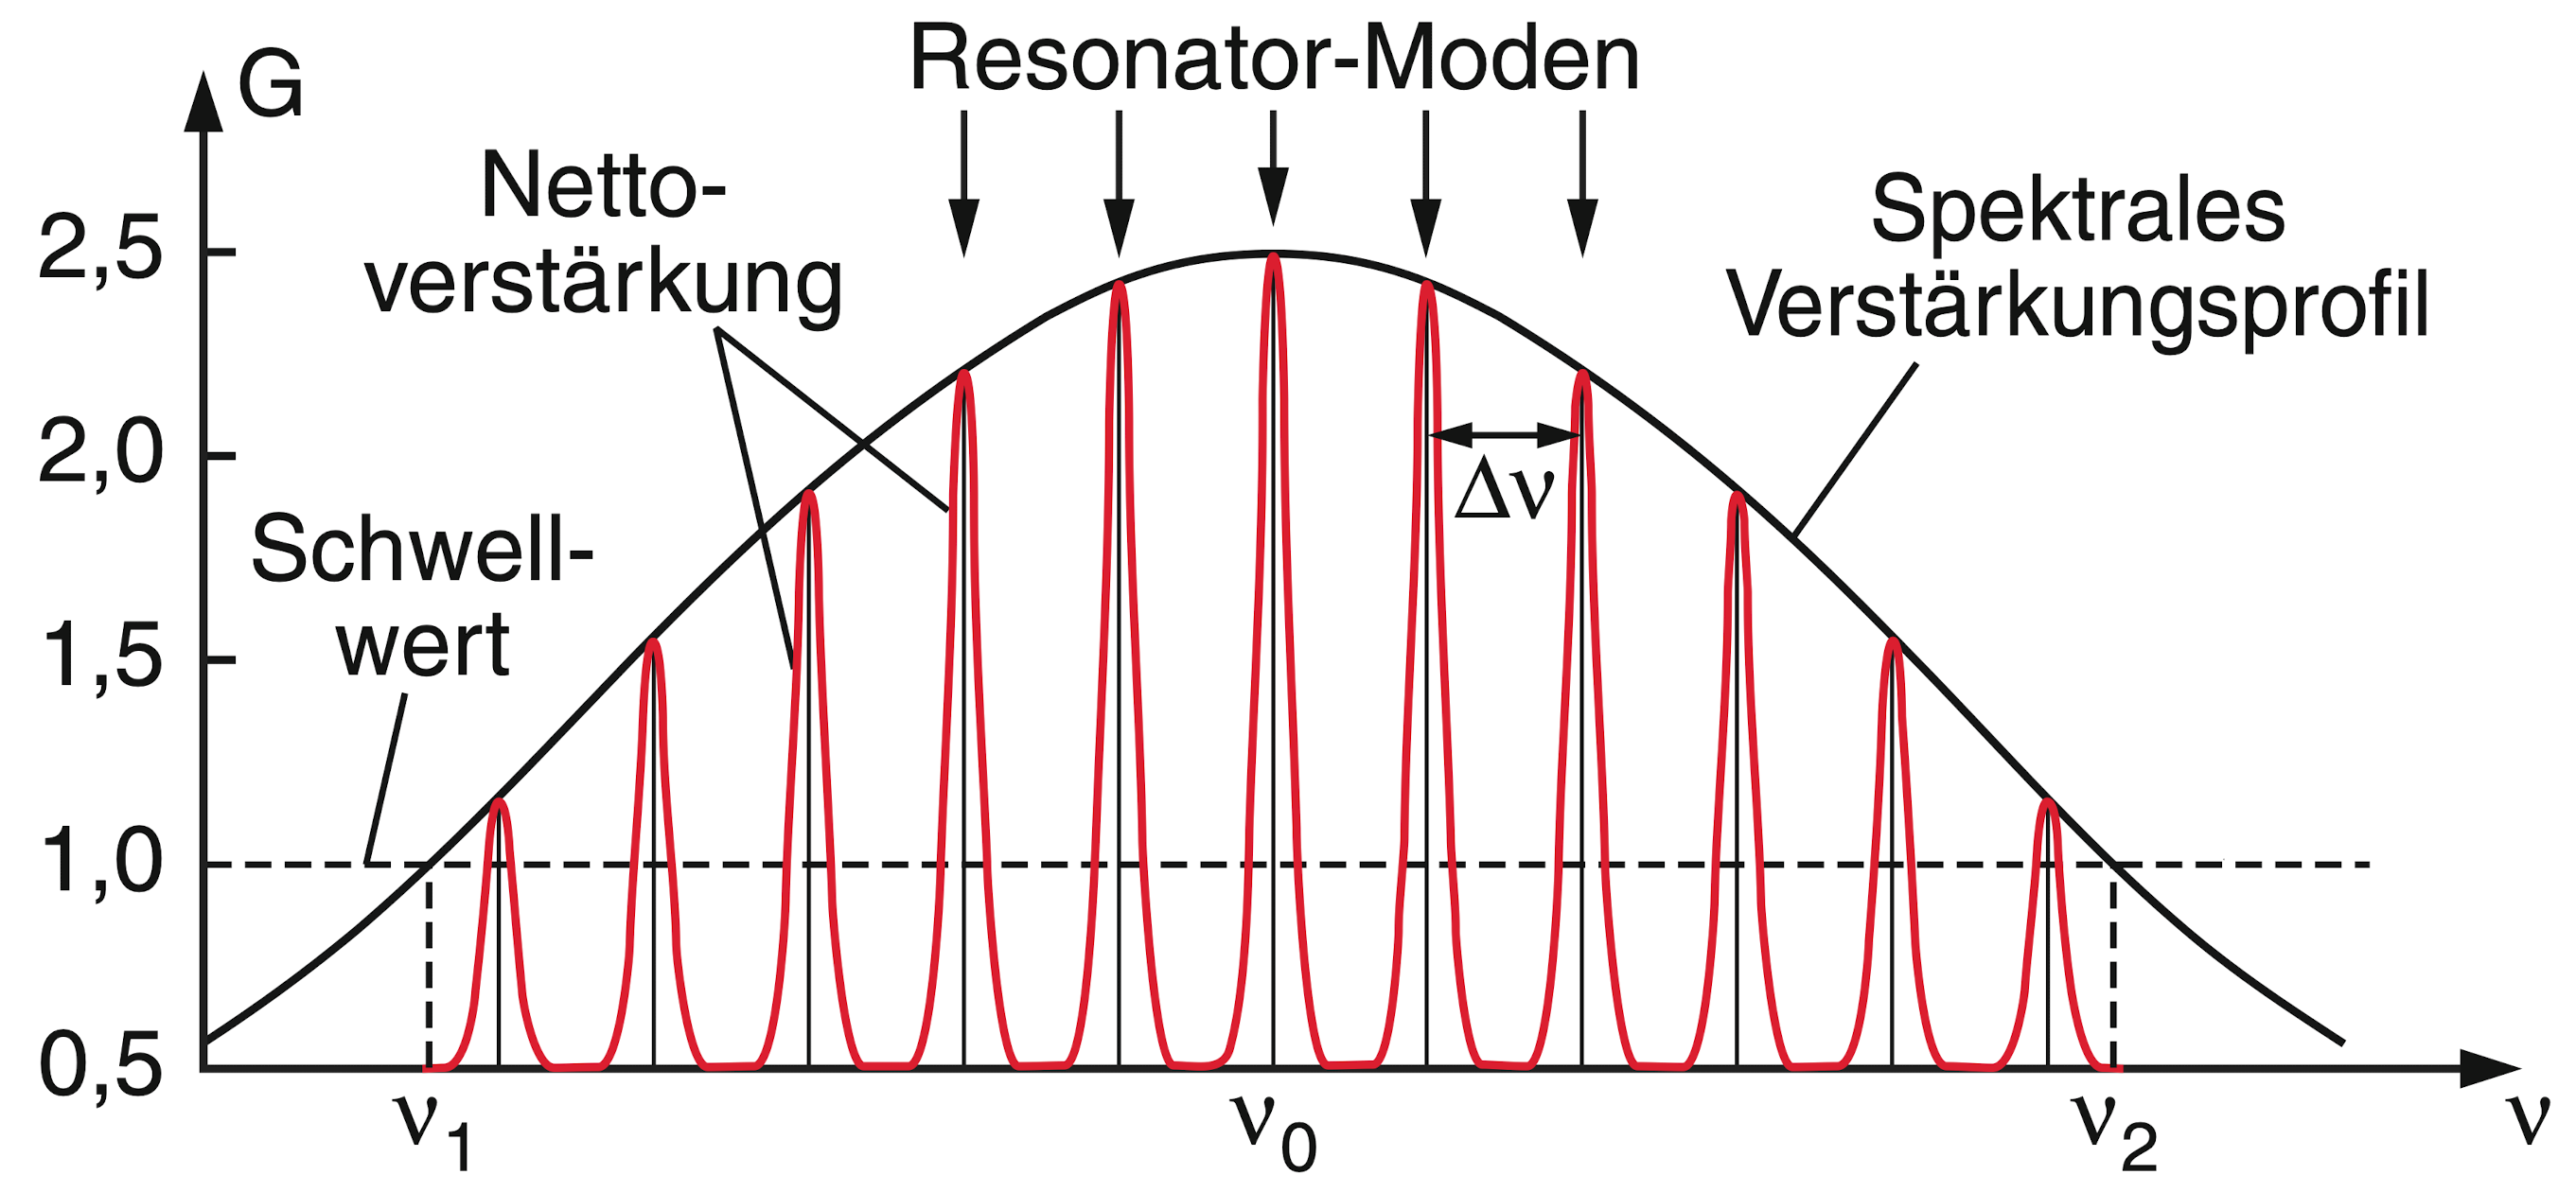
\includegraphics[scale=0.2]{Bilder/Laserprofil.png}
    \captionof{figure}{Nettoverstärkung $G$ innerhalb des dopplerverbreiterten Ver- stärkungsprofils des aktiven Mediums. Die senkrechten schwarzen Linien innerhalb der Resonanzmaxima des Resonators geben die Oszillationsfrequenzen eines Mehrmodenlasers an, bei dem die Transversalmoden unterdrückt wurden \cite{DemtroederAtome}}
    \label{fig:cwlaser}
\end{center}
